\section{Model Results}
	Given a coordinate input of the locations of participants and the time of year, our model optimizes the location for a meeting and predicts the total ticket costs. Since the exact coordinate is not necessarily a city, the nearest city with an airport city was selected as the best location. 

The top coordinates for each scenario are shown, and if a nearby airport exists, it is shown as well.\\


Scenario 1\\
52.1863724, 93.1053239 - Kyzyl Airport, Kyzyl, Russia\\
52.1863724, 88.1053239\\
52.1863724, 98.1053239\\
47.1863724, 88.1053239 - Altay Airport, Altay, Xinjiang, China\\
52.1863724, 103.105324 - International Airport Irkutsk, Irkutsk, Russia\\
47.1863724, 93.1053239\\
52.1863724, 83.1053239\\
47.1863724, 83.1053239 - Tacheng Airport, Tacheng Prefecture, China\\
52.1863724, 108.105324 - Baikal International Airport, Ulan-Ude, Russia\\

Scenario 2\\
52.1863724, 73.9411199 - Astana International Airport, Astana, Kazakhstan\\
52.1863724, 68.9411199 - Kokshetau Airport, Kokshetau, Kazakhstan\\
52.1863724, 78.9411199\\
52.1863724, 63.9411199 - Kostanay Airport, Kostanay, Kazakhstan\\
47.1863724, 73.9411199 - Balkhash Airport, Balkhash, Kazakhstan\\
47.1863724, 78.9411199 - \\
47.1863724, 68.9411199 - Zhezhazgan Airport, Zhezqazgan, Kazakhstan\\

	Typically, the predicted latitudinal coordinate $\approx$ average latitudinal location of the participants. However, the optimal longitudinal location tended towards the western side so that there would be more western travel than eastern travel. In our model, this is due to the dependence of the severity of jet lag begin on direction. Similarly to a study conducted by Lu et al, our model showed that eastward travel caused more loss of productivity from jet lag than westward travel. We conducted a paired t-test to compare the severity of jet lag from eastward travel and westward travel. The severity of jet lag from eastward jet lag was significantly greater than the severity of westward jet lag (\textit{p} = 0.002, df = 58, \textit{t} = 2.00). Locations that required less eastward travel were more optimal. 
	Below is a map of our results and the input for both scenarios. 

\begin{figure}
	\centerline{\includegraphics[width=0.75\textwidth]{scenario1.eps}}
\caption{Above are the model's results for scenario one. We chose the optimal locations by considering the resulting amount of jetlag, distance, and expenses. The most optimal locations, in decreasing order, are Kyzyl, Altay, Irkutsk, Tacheng, Baikal. However, our team recommends we use Irkutsk, due to its relatively high availability of infrastructure.}
\end{figure}

\begin{figure}
	\centerline{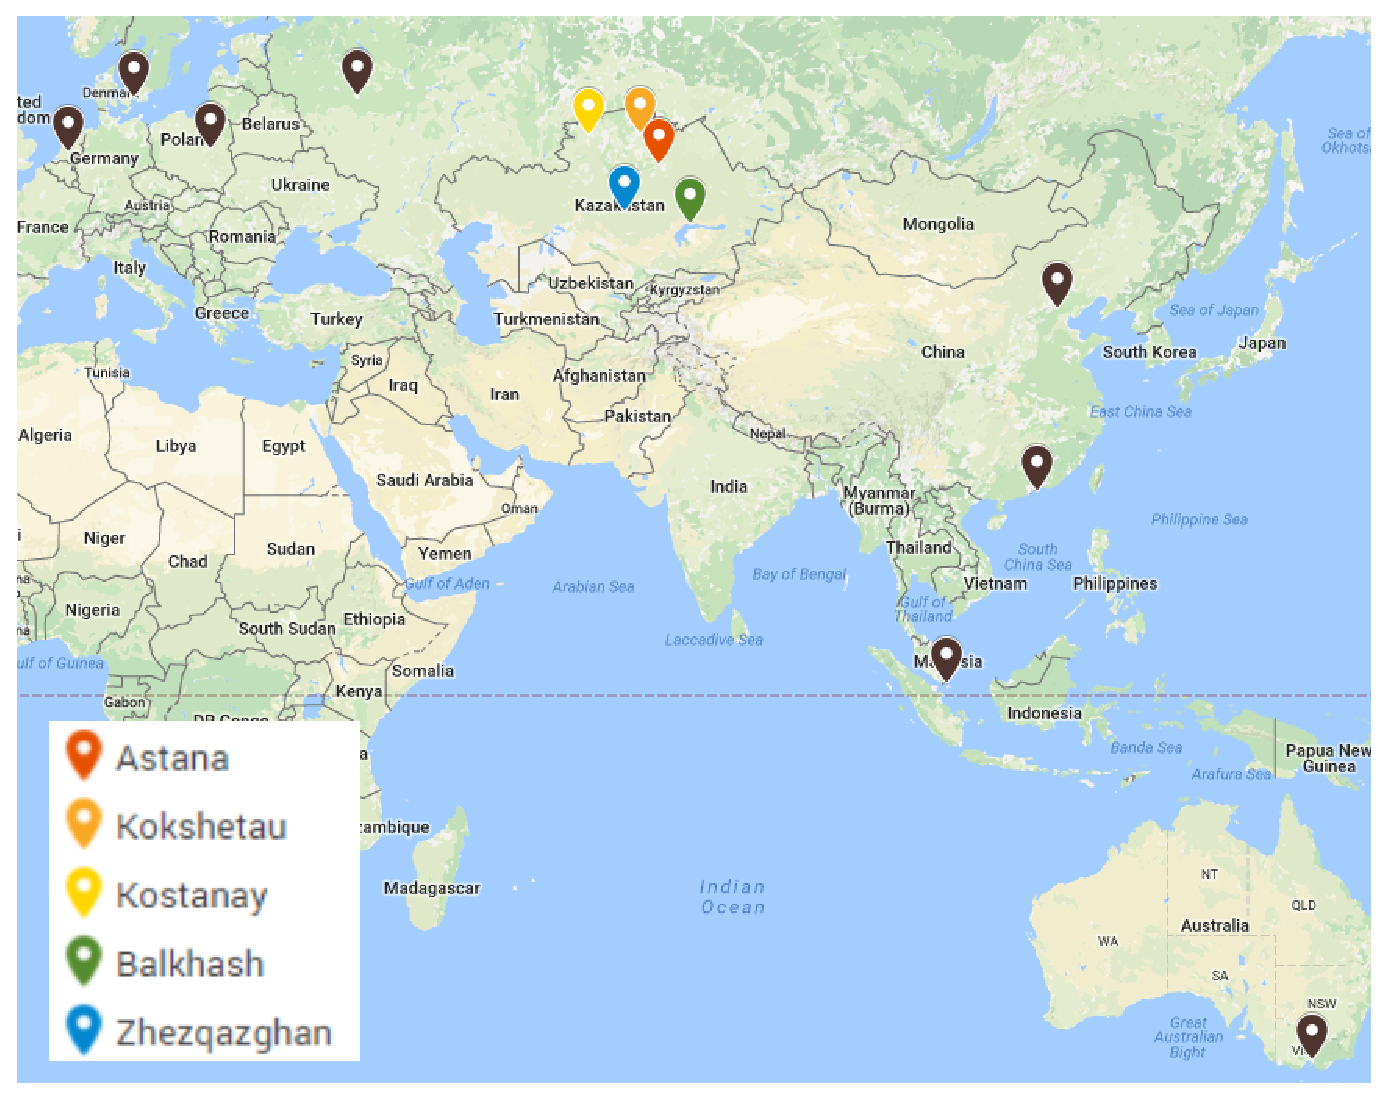
\includegraphics[width=0.75\textwidth]{scenario2.eps}}
\caption{Above are the model's results for scenario two. We chose the optimal locations by considering the resulting amount of jetlag, distance, and expenses. The most optimal locations, in decreasing order, are Astana, Kokshetau, Kostanay, Balkash, Zhezhazgan. Our team recommends we use Astana, due to its relatively high fitness rating.}
\end{figure}


\begin{figure}
	\centerline{\includegraphics[width=\textwidth]{LAXtoNRTprice.eps}}
\caption{Graphed above are the flight cost data and the function our gradient descent polynomial regressor outputted. Note the slight underfit. Our team intentionally prevented the algorithm from fully convergence due to an extreme variance in ticket pricing.}
\end{figure}


\begin{figure}
	\centerline{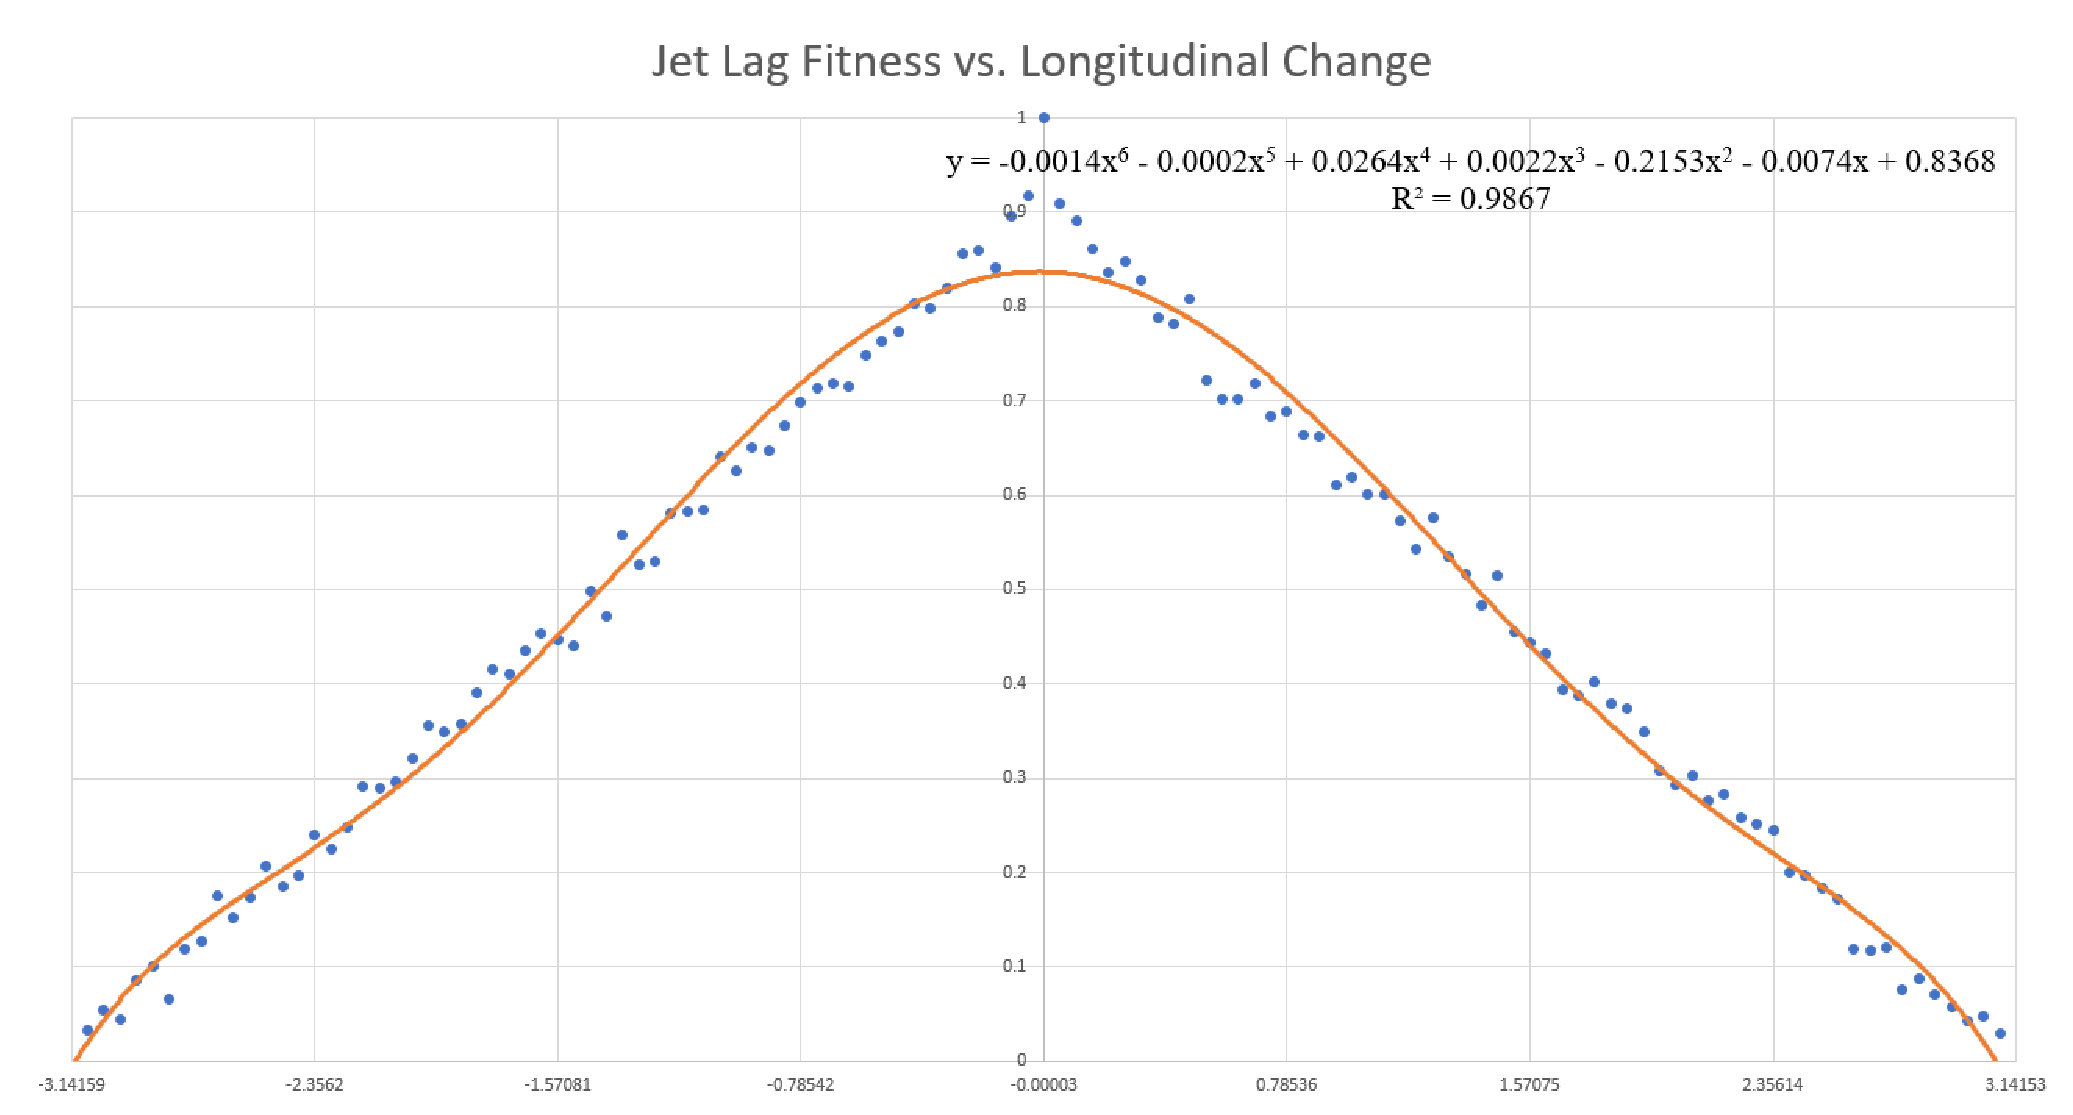
\includegraphics[width=0.75\textwidth]{kuramotofitnessgraph.eps}}
	\caption{Above are the fitness values for certain $\Delta(P)$ that a participant travels. Note that this function is not even and that the results are not strictly decreasing on $[0, \pi]$ and not strictly increasing on $[-\pi, 0]$. In these ranges, a slight change in angle does not gaurantee a predictable change in fitness. As in real life, random chance affected amount of jet lag experienced. Unforutnately, initial conditions such as mood, nutrition, and mental stability, which may vary from person to person, cannot be modeled, and the best way to account for this is to introduce variability in the results. This algorithm is further explained in subsections 3.1 and 4.1}
\end{figure}	
\begin{figure}[t!]
	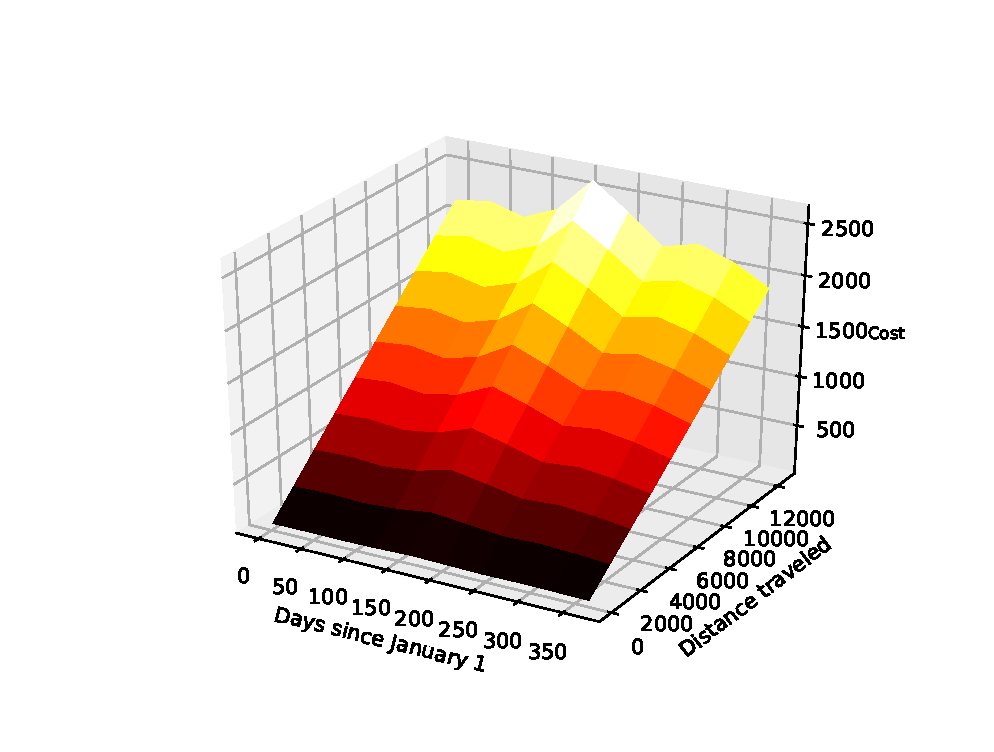
\includegraphics[width=\textwidth]{destination_path.eps}
	\caption{Above is a surface plot of the Number of Days since January 1 and Distance in Miles traveled vs. Ticket Cost}
\end{figure}

\begin{figure}
	\centering{\includegraphics[width=0.5\textwidth]{teamlogo.eps}}
\end{figure}
